\documentclass[border=10pt]{standalone}
\usepackage{tikz}
\usetikzlibrary{arrows.meta, calc}

\begin{document}

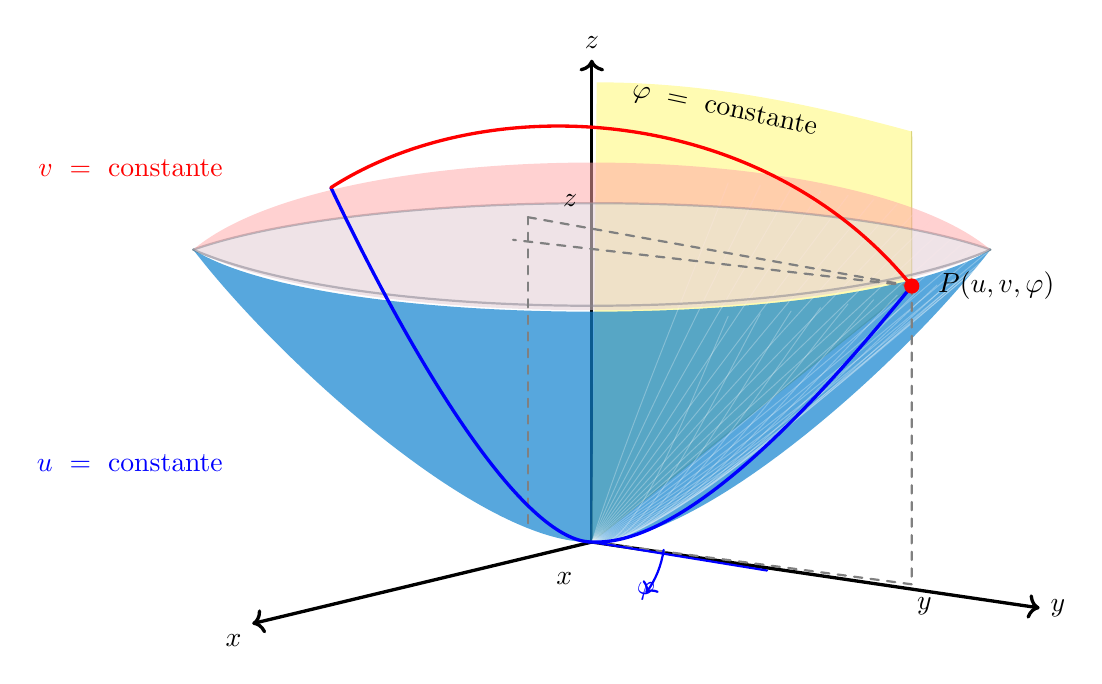
\begin{tikzpicture}[scale=1.25, line cap=round, line join=round]
    \coordinate (O) at (0,-1.05);
    \coordinate (P) at (3.25,1.55);
    \coordinate (L) at (-2.65,2.55);

    % Axes in an oblique 3D view
    \draw[->, very thick] (O) -- (-3.45,-1.88) node[below left] {$x$};
    \draw[->, very thick] (O) -- (4.55,-1.72) node[right] {$y$};
    \draw[->, very thick] (O) -- (0,3.85) node[above] {$z$};

    % Yellow parabolic section plane: phi constant
    \path[fill=yellow!55, opacity=.55]
        (O) -- (P) -- (3.25,3.12)
        .. controls (2.05,3.45) and (1.05,3.62) .. (0.05,3.62)
        -- cycle;
    \draw[yellow!70!black, opacity=.55] (O) -- (P) -- (3.25,3.12);

    % Lower translucent curved paraboloid surface
    \path[fill=cyan!65!blue, opacity=.70]
        (-4.05,1.92)
        .. controls (-3.15,.75) and (-1.10,-1.08) .. (O)
        .. controls (1.10,-1.08) and (3.15,.75) .. (4.05,1.92)
        .. controls (2.70,1.08) and (-2.70,1.08) .. (-4.05,1.92)
        -- cycle;
    \path[fill=cyan!25, opacity=.38]
        (-4.05,1.92)
        .. controls (-2.45,1.10) and (2.45,1.10) .. (4.05,1.92)
        .. controls (2.25,2.55) and (-2.25,2.55) .. (-4.05,1.92)
        -- cycle;

    % Surface rulings on the lower bowl
    \foreach \t in {-70,-65,...,70}{
        \draw[white, opacity=.28, line width=.35pt]
            (O) .. controls ({1.15*cos(\t)},{-.55+0.75*sin(\t)}) and ({2.75*cos(\t)},{.85+0.65*sin(\t)}) .. ({4.05*cos(\t)},{1.92+0.72*sin(\t)});
    }
    \draw[cyan!40!black, opacity=.55, line width=.8pt]
        (-4.05,1.92) .. controls (-2.30,1.16) and (2.30,1.16) .. (4.05,1.92);
    \draw[cyan!40!black, opacity=.55, line width=.8pt]
        (-4.05,1.92) .. controls (-2.25,2.55) and (2.25,2.55) .. (4.05,1.92);

    % Upper translucent curved paraboloid surface
    \path[fill=red!35, opacity=.52]
        (-4.05,1.92)
        .. controls (-2.65,3.10) and (2.65,3.10) .. (4.05,1.92)
        .. controls (2.25,2.55) and (-2.25,2.55) .. (-4.05,1.92)
        -- cycle;
    \path[fill=red!25, opacity=.35]
        (-4.05,1.92)
        .. controls (-2.45,1.10) and (2.45,1.10) .. (4.05,1.92)
        .. controls (2.25,2.55) and (-2.25,2.55) .. (-4.05,1.92)
        -- cycle;

    % Dashed coordinate projections associated with P only
    \draw[dashed, gray, line width=.8pt] (P) -- (3.25,-1.48);
    \draw[dashed, gray, line width=.8pt] (3.25,-1.48) -- (O);
    \draw[dashed, gray, line width=.8pt] (P) -- (-.80,2.02);
    \draw[dashed, gray, line width=.8pt] (-.65,-.86) -- (-.65,2.25);
    \draw[dashed, gray, line width=.8pt] (-.65,2.25) -- (P);

    % Prominent parabolic trace curves through P
    \draw[blue, very thick]
        (L) .. controls (-1.70,.55) and (-.65,-1.05) .. (O)
            .. controls (1.05,-1.10) and (2.55,.70) .. (P);
    \draw[red, very thick]
        (L) .. controls (-1.05,3.58) and (1.75,3.40) .. (P);

    % Point P
    \fill[red] (P) circle (2.2pt);

    % Blue angle construction for phi on the base plane
    \draw[blue, thick] (O) -- (1.78,-1.34);
    \draw[blue, thick, ->] (0.73,-1.13) arc[start angle=-8,end angle=-37,radius=.95];
    \node[blue] at (.55,-1.55) {$\varphi$};

    % Labels
    \node[blue, anchor=east] at (-3.65,-.25) {$u\ =\ \mathrm{constante}$};
    \node[red, anchor=east] at (-3.65,2.75) {$v\ =\ \mathrm{constante}$};
    \node[rotate=-12] at (1.35,3.34) {$\varphi\ =\ \mathrm{constante}$};
    \node[anchor=west] at (3.42,1.55) {$P(u,v,\varphi)$};
    \node at (-.28,-1.42) {$x$};
    \node at (3.38,-1.70) {$y$};
    \node at (-.22,2.42) {$z$};
\end{tikzpicture}

\end{document}
